% frontmatter.tex
% Dieses Werk ist unter einem Creative Commons Namensnennung-Keine kommerzielle Nutzung-Weitergabe 
% unter gleichen Bedingungen 3.0 Deutschland Lizenzvertrag lizenziert. Um die Lizenz anzusehen, gehen Sie bitte 
% zu http://creativecommons.org/licenses/by-nc-sa/3.0/de/ oder schicken Sie einen Brief an 
% Creative Commons, 171 Second Street, Suite 300, San Francisco, California 94105, USA.

\pagestyle{empty}
\frontmatter
\begin{FRONTCOVER}
\begin{titlepage}
\begin{textblock*}{210mm}(0mm,0mm)
   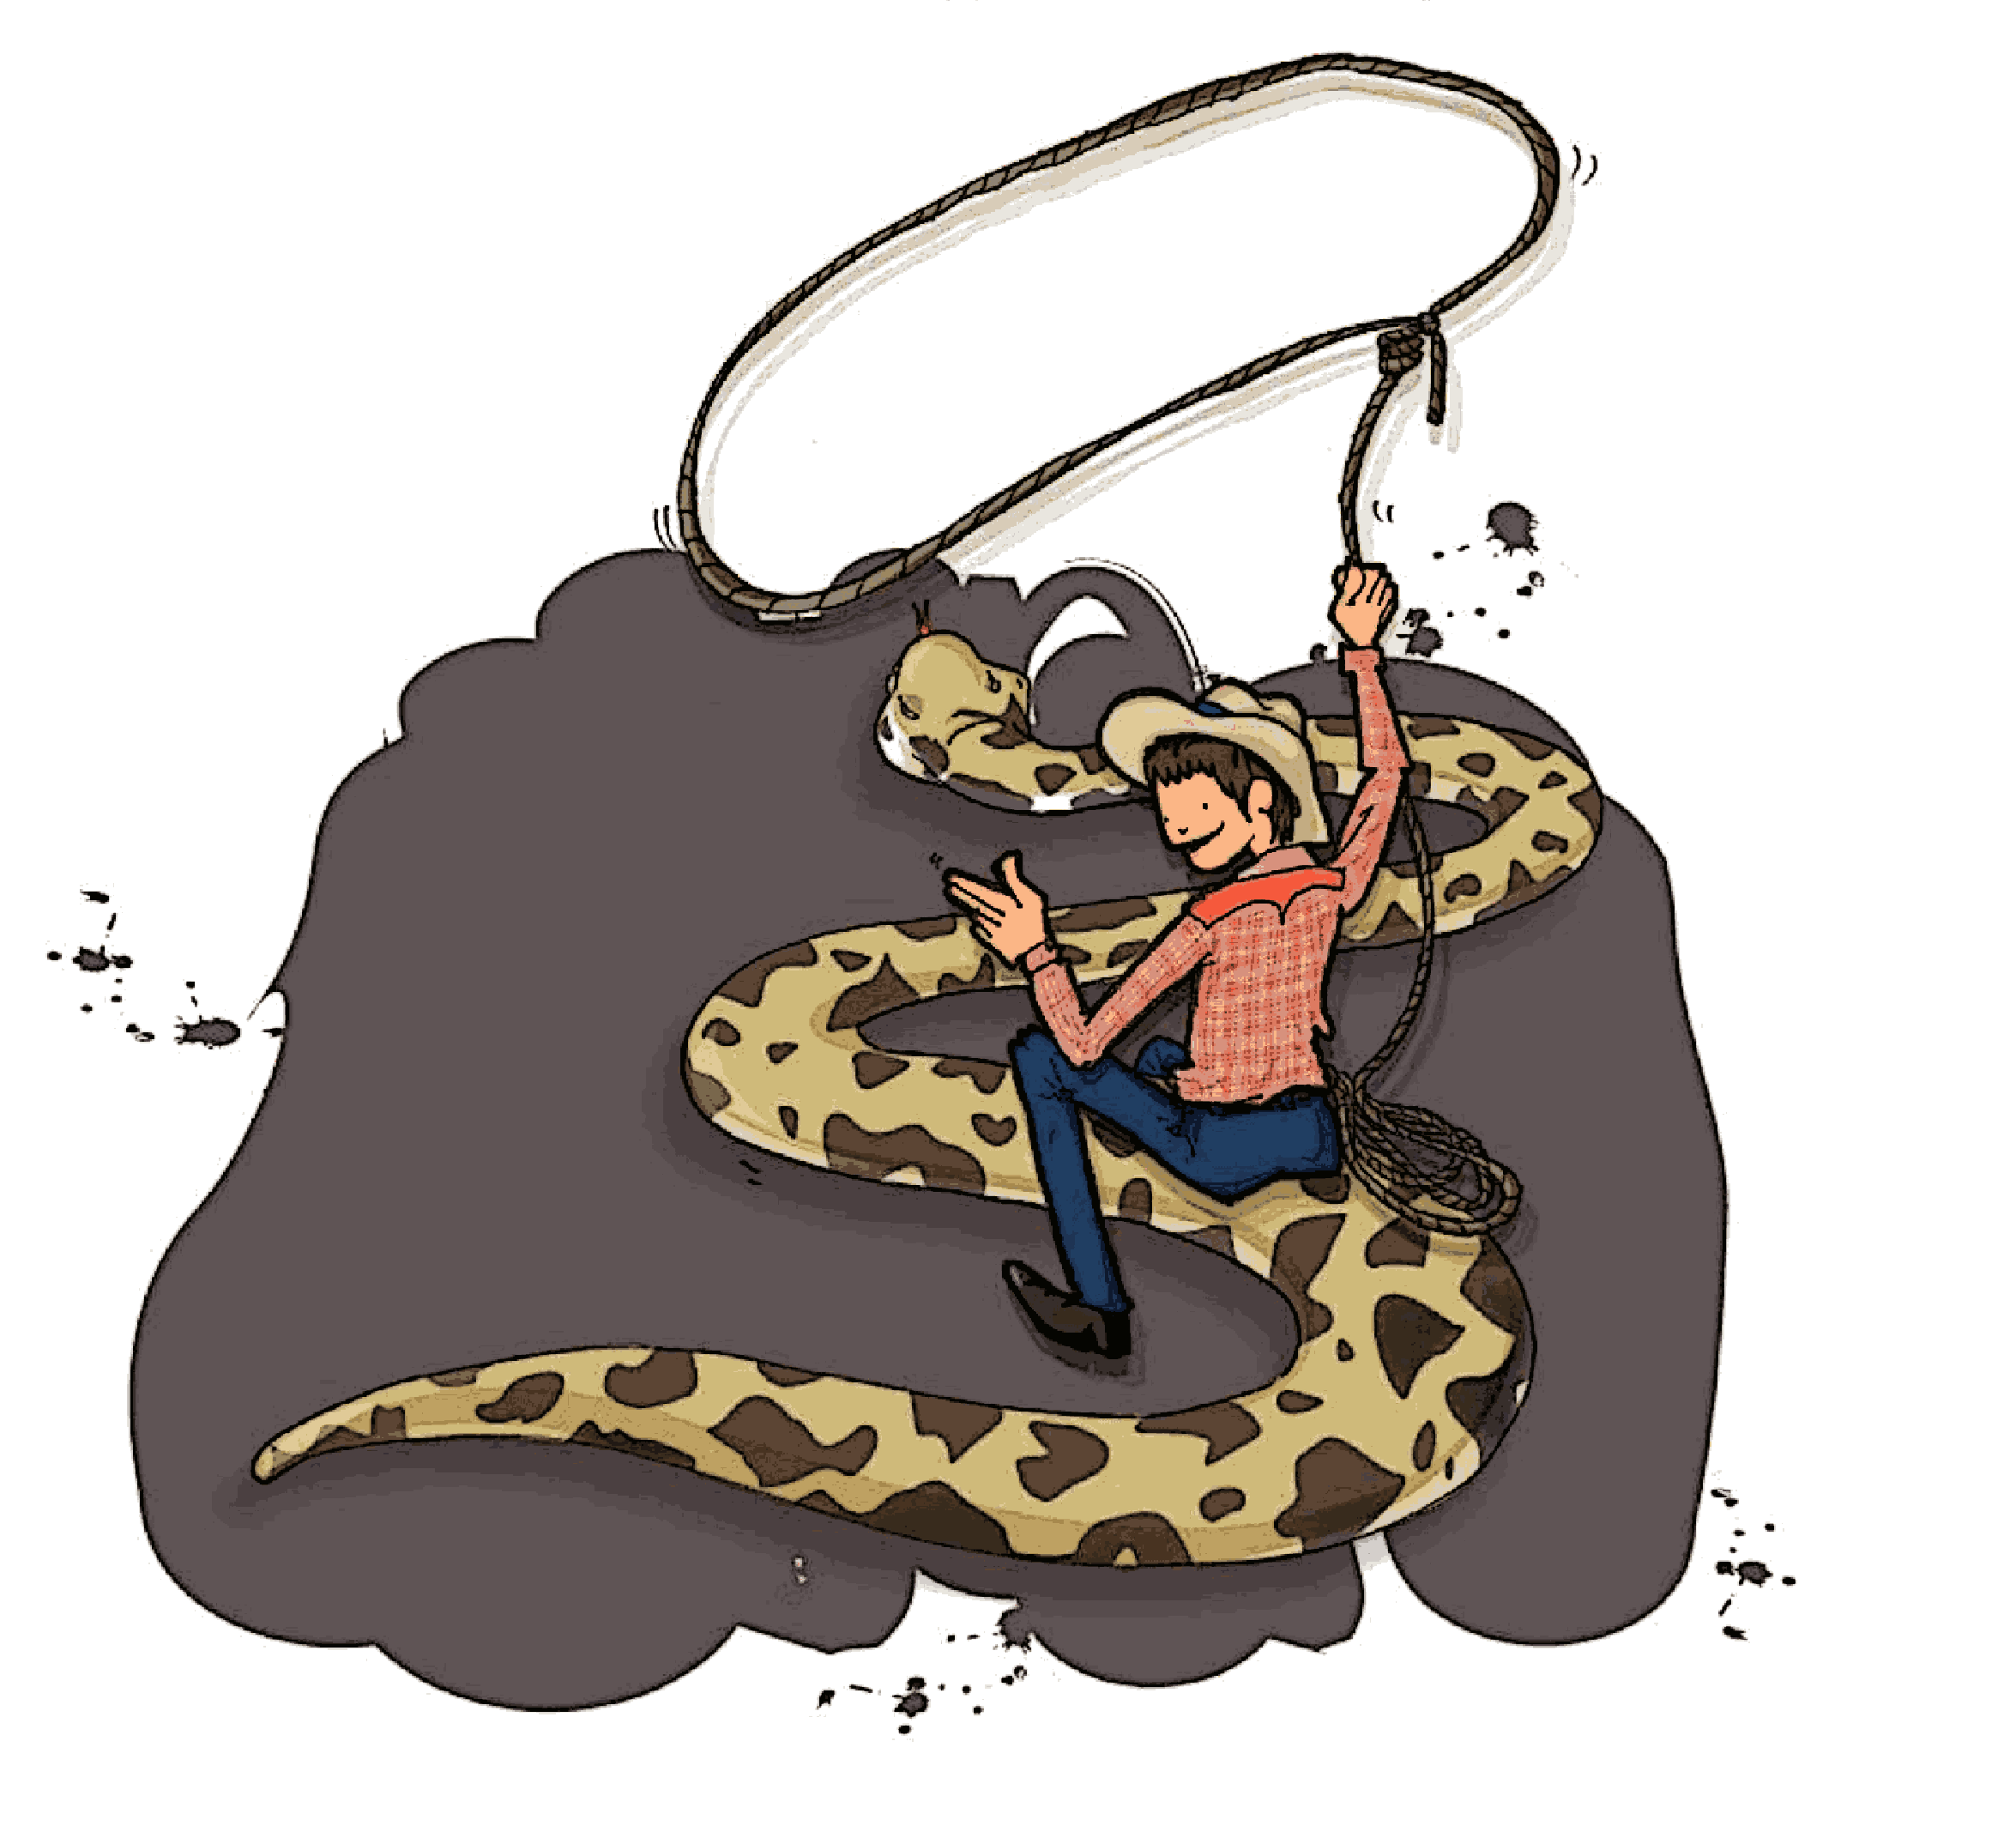
\includegraphics[width=0.9\paperwidth]{cover.eps}
\end{textblock*}
\begin{flushright}
\begin{WINDOWS}
\includegraphics[width=40mm]{windows-edition.eps} 
\end{WINDOWS}
\begin{MAC}
\includegraphics[width=40mm]{mac-edition.eps} 
\end{MAC}
\begin{LINUX}
\includegraphics[width=40mm]{linux-edition.eps} 
\end{LINUX}
\end{flushright}
\end{titlepage}
\end{FRONTCOVER}

\noindent
%\textsf{\emph{Snake Wrangling for Kids, Learning to Program with Python}}\\
\textsf{\emph{Schlangengerangel für Kinder, Programmieren lernen mit Python}}\\
%by Jason R. Briggs\\
von Jason R. Briggs\\
Version 0.7.7
\\
Copyright \copyright 2007.\\
\\
\textsf{\emph{Übersetzung ins Deutsche: Joe Ehrensberger}}\\
Version 0.0.1\\
Copyright der Übersetzung \copyright 2009.\\
Webseite der Übersetzung: \href{http://code.google.com/p/swfk-de}{http://code.google.com/p/swfk-de}\\
\\
%Published by... ah, no one actually.\\
Herausgegeben von... eigenlich Niemanden.\\
\\
%Cover art and illustrations by Nuthapitol C.\\
Umschlaggestaltung und Illustrationen von Nuthapitol C.\\
\linebreak 
\noindent
%Website:\\ \href{http://www.briggs.net.nz/log/writing/snake-wrangling-for-kids}{http://www.briggs.net.nz/log/writing/snake-wrangling-for-kids}\\ 
Webseite:\\ \href{http://www.briggs.net.nz/log/writing/snake-wrangling-for-kids}{http://www.briggs.net.nz/log/writing/snake-wrangling-for-kids}\\ 

\noindent
%Thanks To:\\
Danksagung:\\
%Guido van Rossum (for benevelont dictatorship of the Python language), the members of the \href{http://www.python.org/community/sigs/current/edu-sig/}{Edu-Sig} mailing list (for helpful advice and commentary), author \href{http://www.davidbrin.com/}{David Brin} (the original \href{http://www.salon.com/tech/feature/2006/09/14/basic/}{instigator} of this book), Michel Weinachter (for providing better quality versions of the illustrations), and various people for providing feedback and errata, including: Paulo J. S. Silva, Tom Pohl, Janet Lathan, Martin Schimmels, and Mike Cariaso (among others).  Anyone left off this list, who shouldn't have been, is entirely due to premature senility on the part of the author.\\
An Guido van Rossum (für seine wohlwollende Ditktatur über die Python Sprache), die Mitglieder von der \href{http://www.python.org/community/sigs/current/edu-sig/}{Edu-Sig} Mailing Liste (für den hilfreichen Rat und guten Kommentare), dem Author \href{http://www.davidbrin.com/}{David Brin} (dem Original \href{http://www.salon.com/tech/feature/2006/09/14/basic/}{Impulsgeber} dieses Buches), Michel Weinachter (für das Bereitstellen von Illustrationen von höherer Qualität), und unzählige andere Leute für die Rückmeldungen und Korrekturvorschläge, wie: Paulo J. S. Silva, Tom Pohl, Janet Lathan, Martin Schimmels, und Mike Cariaso (unter anderen).  Falls jemand auf dieser Liste vergessen worden ist, der nicht vergessen werden hätte sollen, so ist dies vollständig der vorzeitigen Senilität des Autors zu verdanken.\\
\noindent
%License:\\
Lizenz:\\
\\
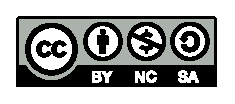
\includegraphics[width=40mm]{by-nc-sa.eps}\\
%This work is licensed under the Creative Commons Attribution-Noncommercial-Share Alike 3.0 New Zealand License. To view a copy of this license, visit\\ \href{http://creativecommons.org/licenses/by-nc-sa/3.0/nz/}{http://creativecommons.org/licenses/by-nc-sa/3.0/nz/} or send a letter to Creative Commons, 171 Second Street, Suite 300, San Francisco, California, 94105, USA.\\
Dieses Werk ist unter einem Creative Commons Namensnennung-Keine kommerzielle Nutzung-Weitergabe unter gleichen Bedingungen 3.0 Deutschland Lizenzvertrag lizenziert. Um die Lizenz anzusehen, gehen Sie bitte zu \\
\href{http://creativecommons.org/licenses/by-nc-sa/3.0/de/}{http://creativecommons.org/licenses/by-nc-sa/3.0/de/} oder schicken Sie einen Brief an Creative Commons, 171 Second Street, Suite 300, San Francisco, California 94105, USA.

\noindent
%Below is a summary of the license.\\
Nachfolgend ist eine Zusammenfassung der Lizenz.\\

\noindent
%You are free:
Sie dürfen:
\begin{itemize}
 %\item \textbf{to Share} — to copy, distribute and transmit the work
 %\item \textbf{to Remix} — to adapt the work
 \item \textbf{Teilen} — das Werk bzw. den Inhalt vervielfältigen, verbreiten und öffentlich zugänglich machen 
 \item \textbf{Verändern} — Abwandlungen und Bearbeitungen des Werkes bzw. Inhaltes anfertigen
\end{itemize}
\noindent
%Under the following conditions:
Zu den folgenden Bedingungen:
\begin{description}
 %\item[Attribution.] You must attribute the work in the manner specified by the author or licensor (but not in any way that suggests that they endorse you or your use of the work).
 %\item[Noncommercial.] You may not use this work for commercial purposes.
 %\item[Share Alike.] If you alter, transform, or build upon this work, you may distribute the resulting work only under the same or similar license to this one.
 \item[Namensnennung] Sie müssen den Namen des Autors/Rechteinhabers in der von ihm festgelegten Weise nennen.
 \item[Keine kommerzielle Nutzung] Dieses Werk bzw. dieser Inhalt darf nicht für kommerzielle Zwecke verwendet werden.
 \item[Weitergabe unter gleichen Bedingungen] Wenn Sie das lizenzierte Werk bzw. den lizenzierten Inhalt bearbeiten oder in anderer Weise erkennbar als Grundlage für eigenes Schaffen verwenden, dürfen Sie die daraufhin neu entstandenen Werke bzw. Inhalte nur unter Verwendung von Lizenzbedingungen weitergeben, die mit denen dieses Lizenzvertrages identisch oder vergleichbar sind.
\end{description}

\noindent
%For any reuse or distribution, you must make clear to others the license terms of this work.\\
Im Falle einer Verbreitung müssen Sie anderen alle Lizenzbedingungen mitteilen, die für dieses Werk gelten.\\

\noindent
%Any of the above conditions can be waived if you get permission from the copyright holder.\\
\textbf{Verzichtserklärung} — Jede der vorgenannten Bedingungen kann aufgehoben werden, sofern Sie die ausdrückliche Einwilligung des Rechteinhabers dazu erhalten. 

\noindent
%Nothing in this license impairs or restricts the author's moral rights.\\
\textbf{Sonstige Rechte} — Die Lizenz hat keinerlei Einfluss auf die folgenden Rechte:
\begin{description}
  \item Die gesetzlichen Schranken des Urheberrechts und sonstigen Befugnisse zur privaten Nutzung;
  \item Das Urheberpersönlichkeitsrecht des Rechteinhabers;
  \item Rechte anderer Personen, entweder am Lizenzgegenstand selber oder bezüglich seiner Verwendung, zum Beispiel Persönlichkeitsrechte abgebildeter Personen.
\end{description}



\vspace*{4cm}
\begin{center}

\includegraphics[width=5cm]{python-powered.eps}
\end{center}

\mainmatter

\pagestyle{plain}

\pagenumbering{roman}
\tableofcontents
